\documentclass[12pt,a4paper]{book}
%\documentclass[a4paper,french]{book}
%\usepackage[17pt]{extsizes}


\input{../1ere-preambule}

\newcommand{\va}[1]{\lvert \ #1 \ \rvert}
\newcommand{\vaf}[1]{\left\lvert \ #1\  \right\rvert}

\begin{document}
\graphicspath{{images/}}
%\setcounter{chapter}{1}
\chapter[Suite arithmétique - Correction des exercices]{Suite arithmétique \\ correction des exercices}
\thispagestyle{fancy}

\subsection*{Ex 11 p 75}


\begin{enumMet}
	\item D’après le graphique, le premier terme $v\left(0\right)=2$.
	
	De plus, $v\left(1\right)=3$ et $v\left(2\right)=4$. Donc $r=v\left(2\right)-v\left(1\right)=4-3=1$.
	
	$v$ est une suite arithmétique de premier terme $v\left(0\right)=2$ et de raison $r=1$.
	\item $v$ étant une suite arithmétique, pour tout entier naturel $n$, on a $v\left(n\right)=r \times n + v\left(0\right)$, soit $v\left(n\right)=1 \times n + 2=n+2$.
\end{enumMet}

\subsection*{Ex 12 p 75}

D'après le graphique, le premier terme $u\left(0\right)=10$.

Pour tout entier naturel $n$, on a $u\left(n\right)=r \times n + u\left(0\right)$, soit $u\left(n\right)=r \times n + 10$.

De plus, $u\left(5\right)=0$. 

Donc : $0=r \times 5 + 10 \Leftrightarrow 5r+10=0 \Leftrightarrow 5r=-10 \Leftrightarrow r=-2$.

En conclusion, $u$ est une suite arithmétique de premier terme $u\left(0\right)=10$ et de raison $r=-2$.

\subsection*{Ex 13 p 75}

Pour tout entier naturel $n$, on a $u\left(n+1\right)=u\left(n\right)-5$.

Donc $u\left(3\right)=u\left(2\right)-5=-7-5=-12$ et $u\left(4\right)=u\left(3\right)-5=-12-5=-17$.

\subsection*{Ex 14 p 75}

Pour tout entier naturel $n$, on a $u\left(n+1\right)=u\left(n\right)+4$.

Donc $u\left(4\right)=u\left(3\right)+4=7+4=11$ et $u\left(5\right)=u\left(4\right)+4=11+4=15$.

Le terme de rang 5 de la suite $u$ est donc $u\left(5\right)=15$.

\subsection*{Ex 15 p 75}

Le terme de rang 9 est $v\left(9\right)=-3 \times 9=-27$.

\subsection*{Ex 16 p 75}

Le cinquième terme est $w\left(4\right)=\dfrac{4}{2}-1=2-1=1$.

\subsection*{Ex 17 p 75}

Les trois premiers termes de la suite $u$ sont $u\left(0\right)=7-6\times 0=7$, $u\left(1\right)=7-6\times 1=1$ et $u\left(2\right)=7-6\times 2=-5$.

\subsection*{Ex 18 p 75}

Pour tout entier naturel $n$, on a $u\left(n\right)=r \times n + u\left(0\right)$, soit $u\left(n\right)=0,25 \times n -3$.

Les trois premiers termes de la suite $u$ sont $u\left(0\right)=0,25 \times 0 -3=-3$, $u\left(1\right)=0,25 \times 1 -3=-2,75$ et $u\left(2\right)=0,25 \times 2 -3=-2,5$.

\subsection*{Ex 19 p 75}


\begin{enumMet}
	\item Le temps écoulé prend des valeurs entières puisque le relevé a lieu toutes les secondes. L’augmentation de la quantité d’eau écoulée chaque seconde est constante.
	
	On peut ainsi modéliser cette situation par une suite $d$ de raison $r=20$ et de premier terme $d\left(0\right)=0$.
	\item Pour tout entier naturel $n$, on a $d\left(n\right)=r \times n + d\left(0\right)$, soit $d\left(n\right)=20 \times n +0=20n$.
	
	Donc $d\left(11\right)=20 \times 11=220$.
	
	Au bout de 11 secondes, la quantité d’eau écoulée est de 220 cL.
\end{enumMet}

\subsection*{Ex 20 p 75}


\begin{enumMet}
	\item  
	\begin{enumMet}
		\item Le nombre d’années écoulées depuis 2021 est un entier naturel. L’augmentation du nombre d’habitants par année est constante. La situation peut donc être modélisée par une suite arithmétique $h$ de raison $r=15$ et de premier terme $h\left(0\right)=1649$.
		\item Pour tout entier naturel $n$, on a $h\left(n\right)=r \times n + h\left(0\right)$, soit $h\left(n\right)=15 \times n +1649$.
	\end{enumMet}
	\item On a $h\left(1\right)=15 \times 1 +1649=1664$. Ce village comptera 1664 habitants en 2022.
	
	On a $h\left(2\right)=15 \times 2 +1649=1679$. Ce village comptera 1679 habitants en 2023.
	
	On a $h\left(3\right)=15 \times 3 +1649=1694$. Ce village comptera 1694 habitants en 2024.
	
	On a $2030=2021+9$.
	
	Donc $h\left(9\right)=15 \times 9 +1649=1784$. Ce village comptera 1784 habitants en 2030.
\end{enumMet}

\subsection*{Ex 33 p 78}

Les nuages de points vert et rouge représentent des phénomènes discrets à croissance linéaire, puisque les points sont alignés.

\subsection*{Ex 34 p 78}

On peut modéliser cette situation par une suite arithmétique puisque l’écart entre deux valeurs consécutives est constant et égal à 10. Cette suite est en revanche finie car il ne peut pas indéfiniment baisser la charge de sa barre de musculation.

\subsection*{Ex 35 p 78}

On ne peut pas modéliser cette situation par une suite arithmétique puisque l’écart entre deux valeurs consécutives n’est pas constant. En effet, $122-156=-34$ et $86-122=-36$.

\subsection*{Ex 36 p 78}


\begin{enumMet}
	\item On a $u\left(0\right)=2 \times 0^2-1=-1$, $u\left(1\right)=2 \times 1^2-1=1$ et $u\left(2\right)=2 \times 2^2-1=7$.
	
	Donc $u\left(1\right)-u\left(0\right)=2$ et $u\left(2\right)-u\left(1\right)=6$.
	
	L’écart entre deux valeurs consécutives de la suite n’est pas constant ($2 \neq 6$). $u$ n’est pas à croissance linéaire.
	\item Pour tout entier naturel $n$, on a $v\left(n+1\right)-v\left(n\right)=\dfrac{\left(n+1\right)+2}{3}-\dfrac{n+2}{3}$ 
	
	$=\dfrac{n+3}{3}-\dfrac{n+2}{3}$
	
	$=\dfrac{1}{3}$.
	
	Ainsi, pour tout entier naturel $n$, $v\left(n+1\right)-v\left(n\right)$ est constant.
	
	$v$ est donc une suite à croissance linéaire.
	
	
	
	$v$ est ainsi une suite arithmétique de raison $r=\dfrac{1}{3} >0$. $v$ est strictement croissante.
\end{enumMet}

\subsection*{Ex 37 p 78}


\begin{enumMet}
	\item L’écart entre deux valeurs consécutives est constant et égal à $-6$.
	
	Or, $58-6=52$.
	
	Le mois suivant, il y aura donc 52 chèvres. 
	\item L’écart entre deux valeurs consécutives est constant et égal à $4$.
	
	Or, $27+4=31$.
	
	Les dix minutes suivantes, 31 mm seront relevés.
\end{enumMet}

\subsection*{Ex 38 p 78}


\begin{enumMet}
	\item L’écart entre deux valeurs consécutives est constant et égal à $-0,4$.
	
	La raison de cette suite est donc $r=-0,4$.
	
	On observe que $r<0$. La suite est donc strictement décroissante.
	\item L’écart entre deux valeurs consécutives est constant et égal à $\dfrac{2}{5}$.
	
	La raison de cette suite est donc $r=\dfrac{2}{5}$.
	
	On observe que $r>0$. La suite est donc strictement croissante.
\end{enumMet}

\subsection*{Ex 39 p 78}


\begin{enumMet}
	\item On a $u\left(10\right)=5 \times 10 -12=38$.
	\item On a $u\left(10\right)=\dfrac{4\times 10 +7}{3}=\dfrac{47}{3}$.
\end{enumMet}

\subsection*{Ex 40 p 78}

On a $u\left(2\right)=u\left(1\right)+0,1=0,2+0,1=0,3$ ;

$u\left(3\right)=u\left(2\right)+0,1=0,3+0,1=0,4$ ;

et $u\left(4\right)=u\left(3\right)+0,1=0,4+0,1=0,5$.



La raison de la suite $u$ est $r=0,1 >0$. $u$ est donc strictement croissante.

\subsection*{Ex 41 p 78}

L’écart entre deux valeurs consécutives est constant et égal à $-\dfrac{3}{4}$, puisque $$\dfrac{5}{2}-\dfrac{13}{4}=\dfrac{7}{4}-\dfrac{5}{2}=1-\dfrac{7}{4}=\dfrac{1}{4}-1=-\dfrac{3}{4}.$$

La raison de cette suite est donc $r=-\dfrac{3}{4}$.

Les deux termes suivants sont donc $\dfrac{1}{4}-\dfrac{3}{4}=-\dfrac{1}{2}$ et $-\dfrac{1}{2}-\dfrac{3}{4}=-\dfrac{5}{4}$.

\subsection*{Ex 42 p 78}

$u$ est une suite arithmétique de raison 3 donc, pour tout entier naturel $n$, $u\left(n+1\right) = u\left(n\right)+3$.

On a donc $u\left(7\right)=u\left(6\right)+3=-4+3=-1$ et $u\left(8\right)=u\left(7\right)+3=-1+3=2$.

\subsection*{Ex 43 p 78}

Pour tout entier naturel $n$, on a $u\left(n\right)= r \times n + u\left(0\right)$.
\begin{enumerate}[label=\arabic*.]
	\item Dans cette question, $u\left(n\right)= -7 \times n + 3$.
	
	Ainsi, $u\left(5\right)= -7 \times 5 + 3=-32$.
	\item Dans cette question, $u\left(n\right)= -1,2 \times n + 5,6$.
	
	Ainsi, $u\left(5\right)= -1,2 \times 5 + 5,6=-0,4$.
\end{enumerate}

\subsection*{Ex 44 p 78}

Voici le nuage des cinq premiers points de chacune des suites données.
\begin{enumerate}[label=\arabic*.]
	\item On calcule les cinq premiers termes de la suite.
	
	$u\left(0\right)= 2- 5 \times 0 =2$ ; $u\left(1\right)= 2- 5 \times 1 =-3$ ; $u\left(2\right)= 2- 5 \times 2 =-8$ ; $u\left(3\right)= 2- 5 \times 3 =-13$ et $u\left(4\right)= 2- 5 \times 4 =-18$.
	
	
	\begin{center}
		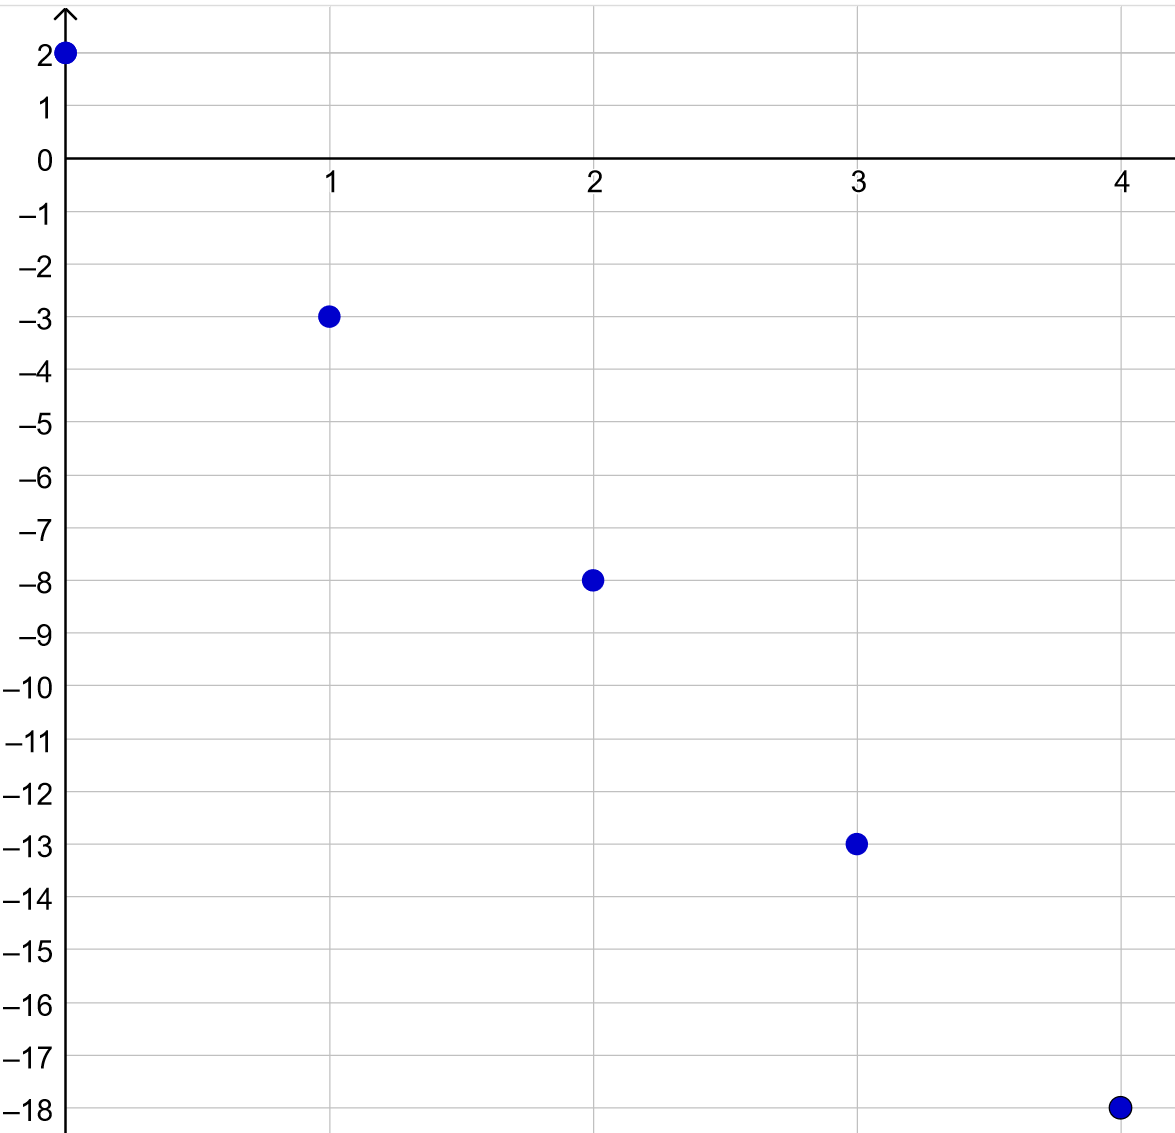
\includegraphics[scale = 0.24]{images/image4.png}
	\end{center}
	
	\item On détermine les cinq premiers termes de la suite. On a déjà $w\left(0\right)=3$.
	
	On calcule les autres termes : $w\left(1\right)= w\left(0\right)-2=3-2=1$ ; $w\left(2\right)= w\left(1\right)-2=1-2=-1$ ; $w\left(3\right)= w\left(2\right)-2=-1-2=-3$ et $w\left(4\right)= w\left(3\right)-2=-3-2=-5$.
	
	
	\begin{center}
		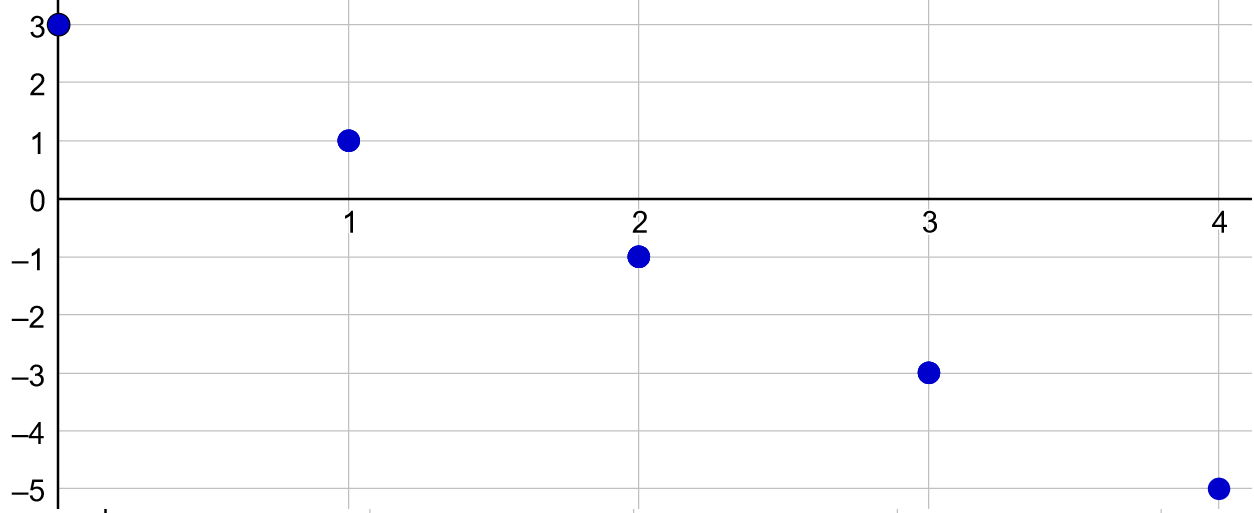
\includegraphics[scale = 0.25]{images/image6.png}
	\end{center}
	
\end{enumerate}

\subsection*{Ex 45 p 79}

$u$ est une suite arithmétique de raison $r$. Donc $u\left(2\right) = u\left( 1 \right)+r$, $u\left(3\right) = u\left(2\right) + r = u\left(1\right) +2r$, $u\left(4\right) = u\left(3\right) + r = u\left(1\right)+3r$ et enfin $u\left(5\right) = u\left(4\right)+r = u\left(1\right)+4r$. 

D’après le graphique, on a $u\left(1\right)=0$ et $u\left(5\right)=-1$. Donc $-1= 0+4r$, soit $r=-\dfrac{1}{4}$.

La suite $u$ étant une suite arithmétique de raison $r=-\dfrac{1}{4}$, on a, pour tout entier naturel $n$, $u\left(n+1\right)=u\left(n\right)-\dfrac{1}{4}$. En particulier, $u\left(1\right)=u\left(0\right))-\dfrac{1}{4}$ d’où $0 = u\left(0\right)-\dfrac{1}{4}$. D’où $u\left(0\right) = \dfrac{1}{4}$.

En conclusion, pour tout entier naturel $n$, $u\left(n\right) = \dfrac{1}{4}-\dfrac{1}{4}n$.

\end{document}

